\appendix

\chapter{Documentation of ADCP Matrices }
The documentation of all ADCP matrices was captured as screen shots from the official ADCP user guide from Rowe Tech. Inc. \cite{adcp_def} .

\begin{figure}[ht]
\centering
      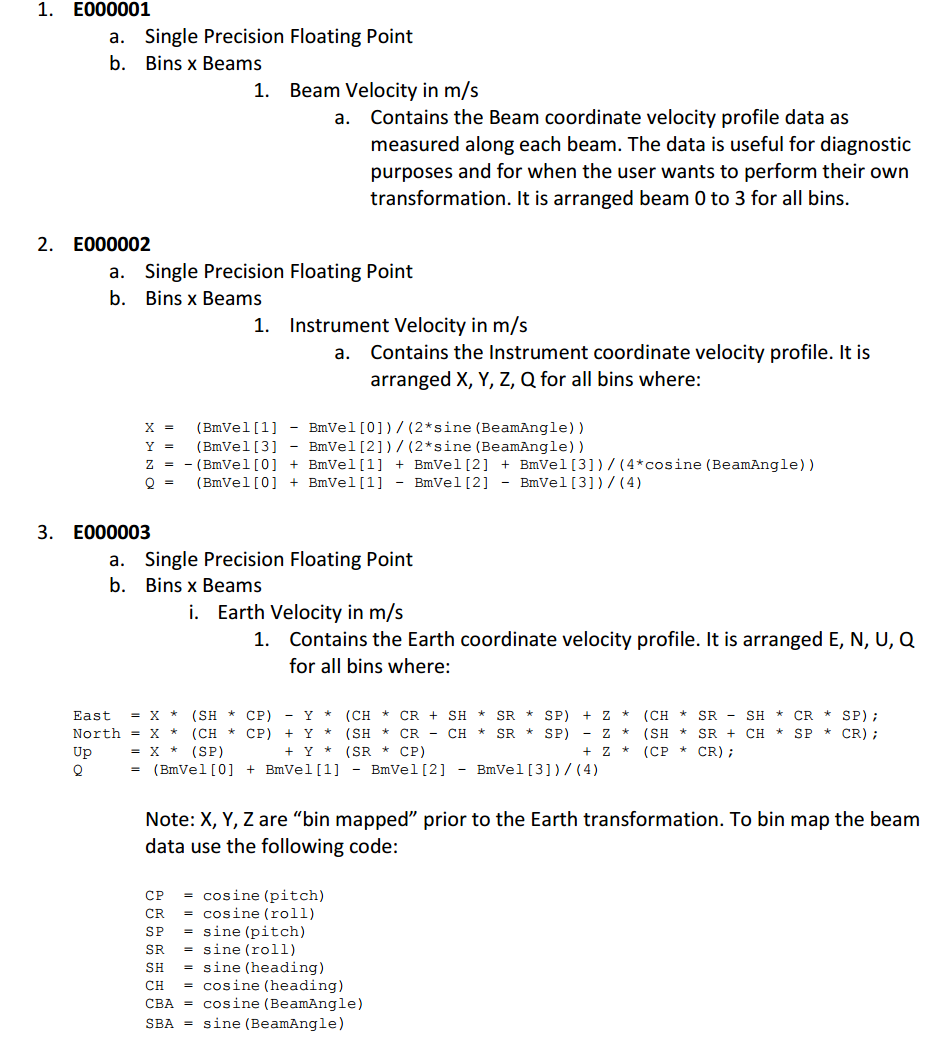
\includegraphics[width=1\textwidth]{ens1}
\end{figure}
\begin{figure}[ht]
\centering
      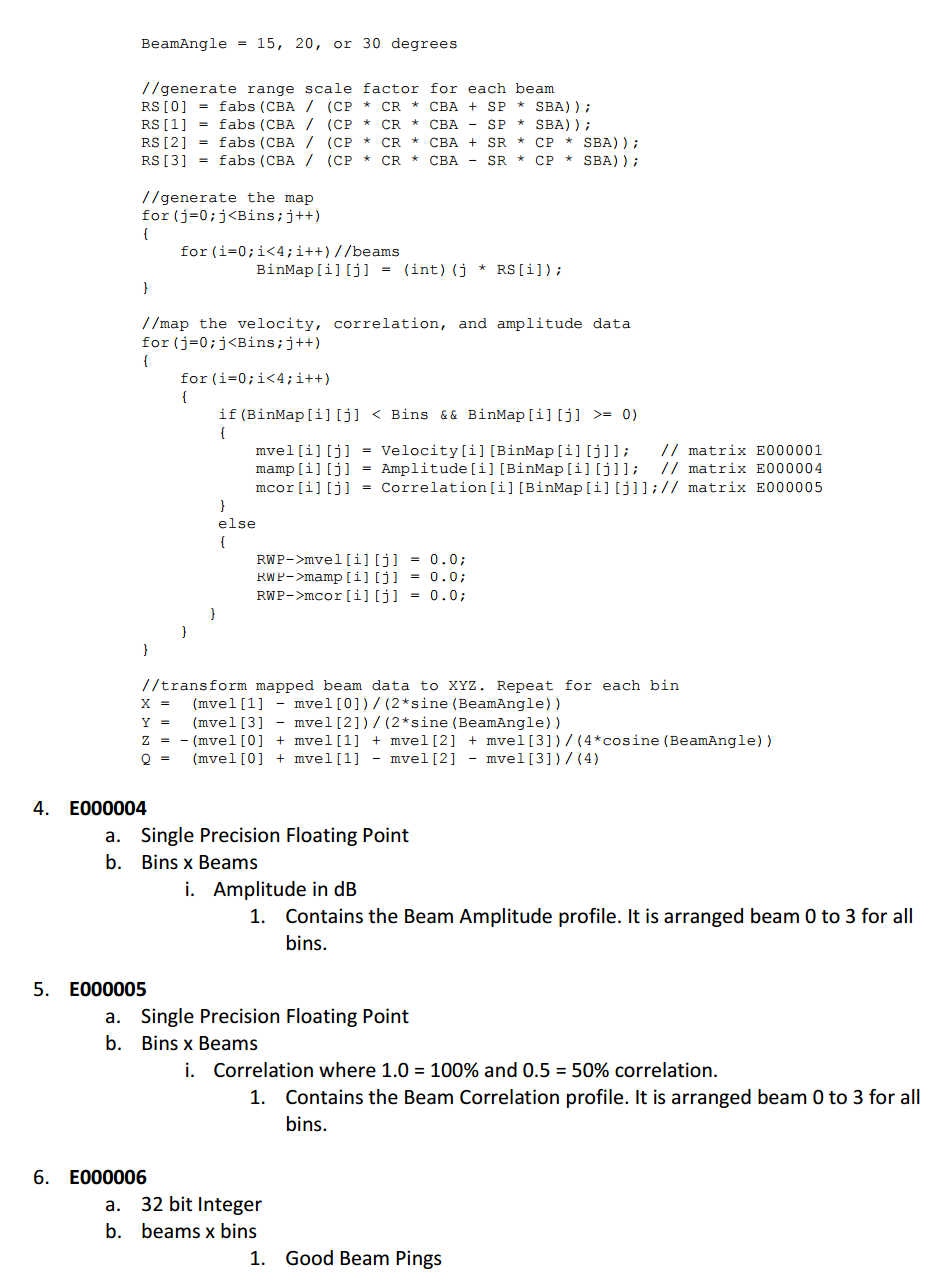
\includegraphics[width=1\textwidth]{ens2}
\end{figure}
\begin{figure}[ht]
\centering
      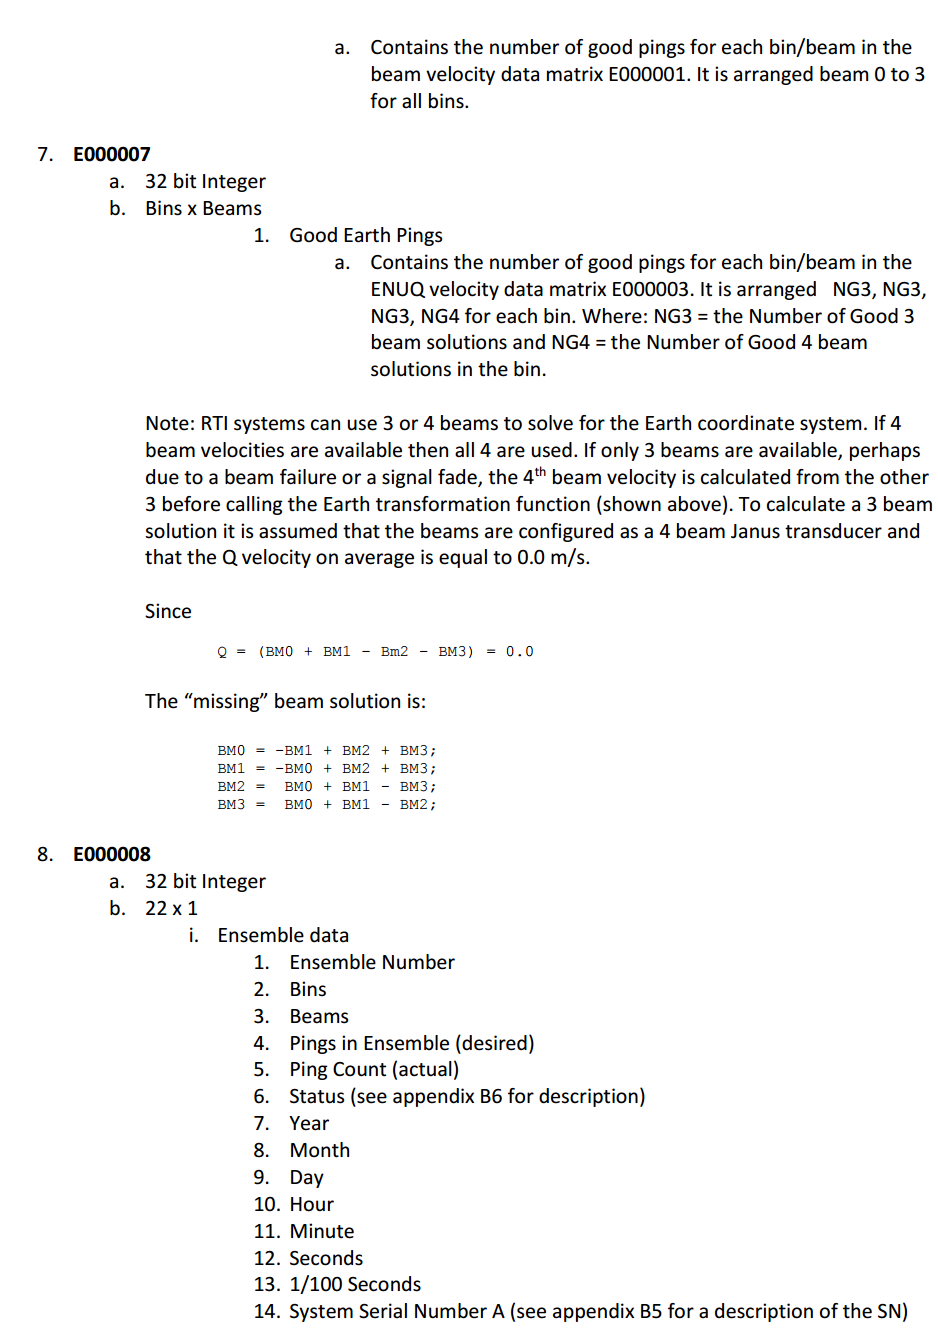
\includegraphics[width=1\textwidth]{ens3}
\end{figure}
\begin{figure}[ht]
\centering
      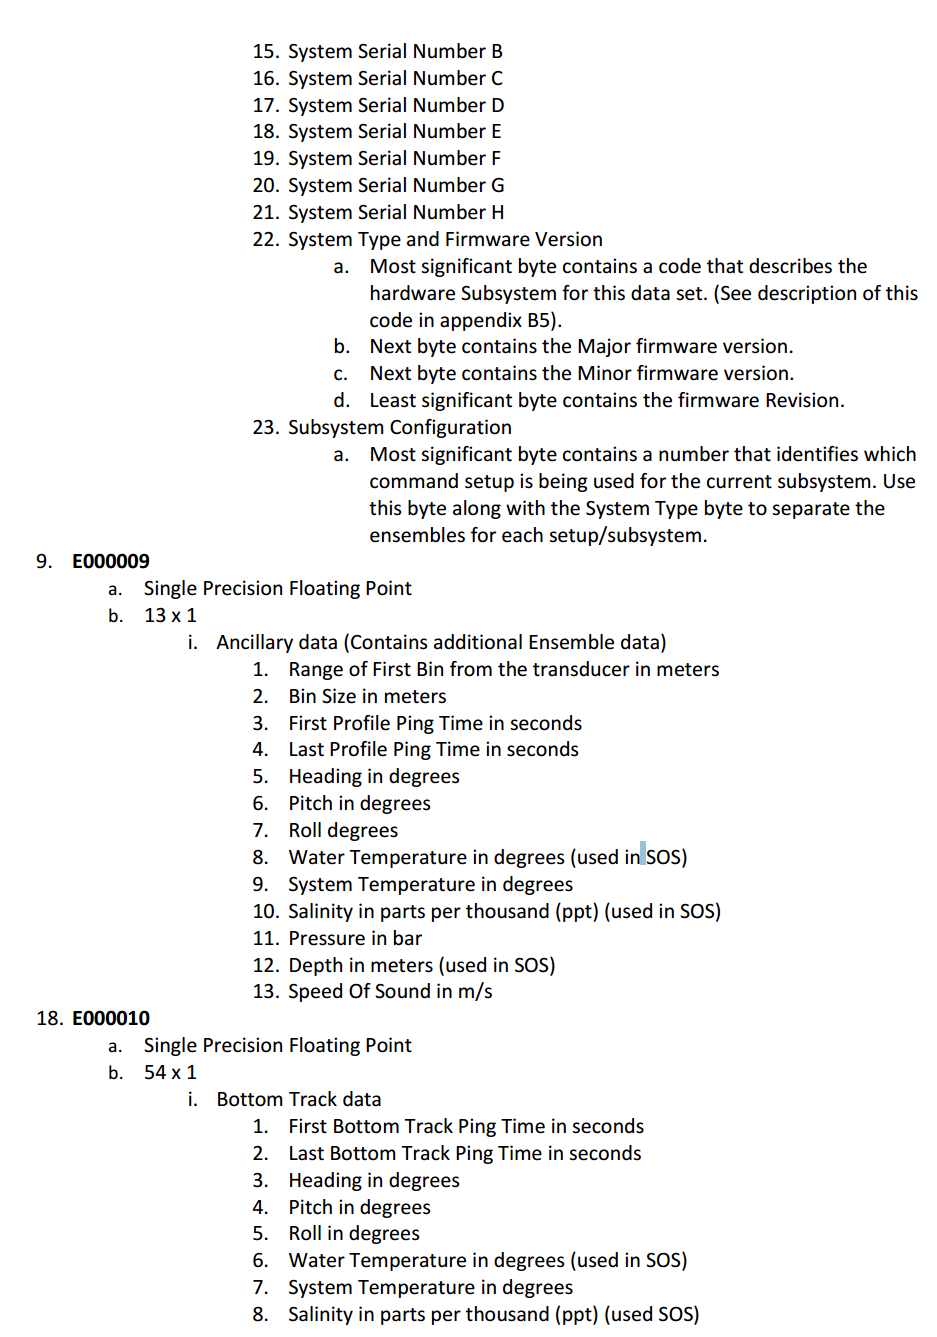
\includegraphics[width=1\textwidth]{ens4}
\end{figure}
\begin{figure}[ht]
\centering
      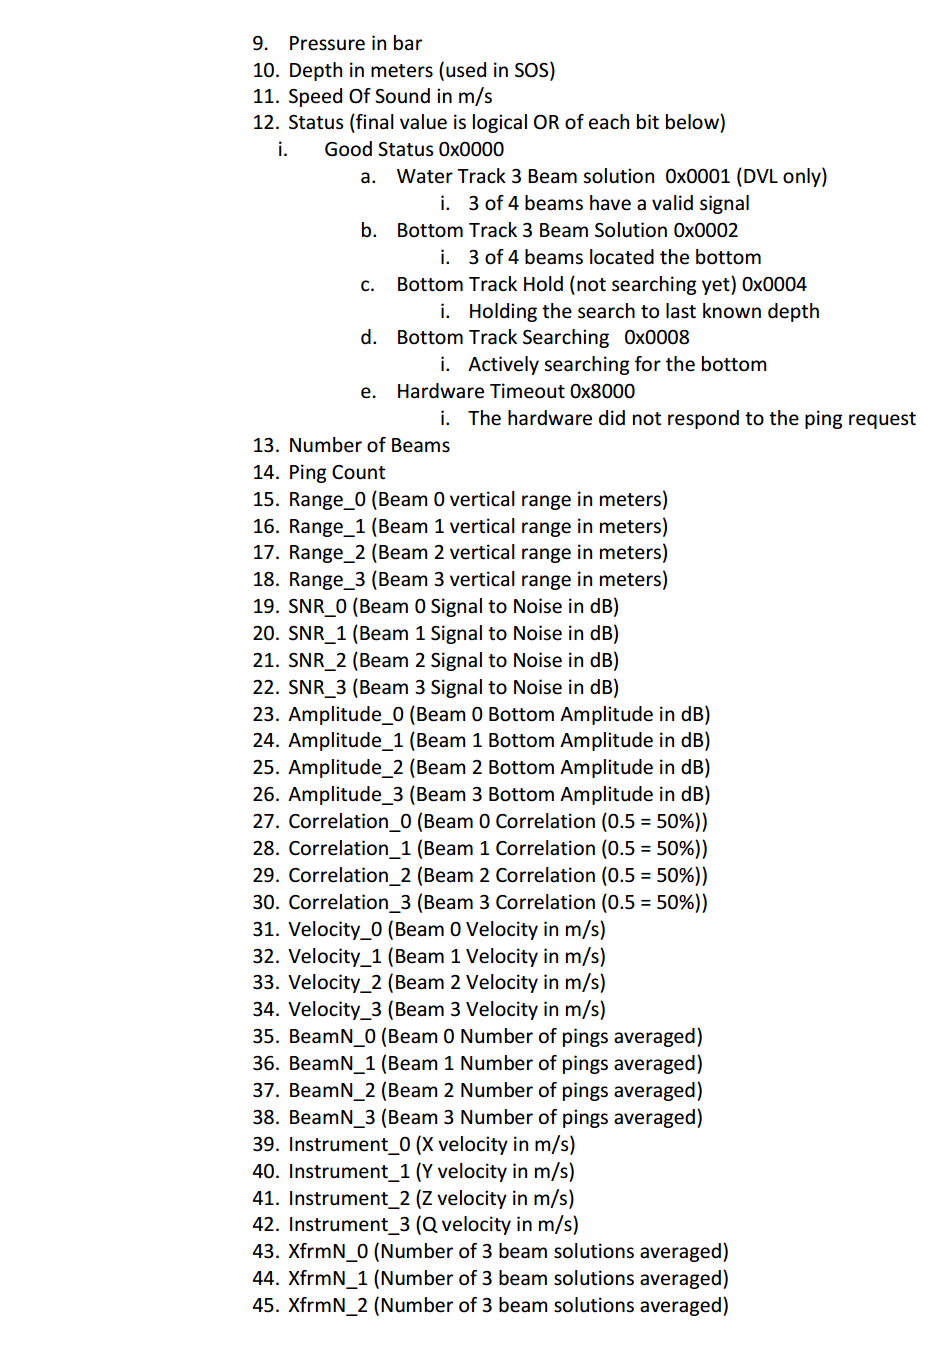
\includegraphics[width=1\textwidth]{ens5}
\end{figure}
\begin{figure}[ht]
\centering
      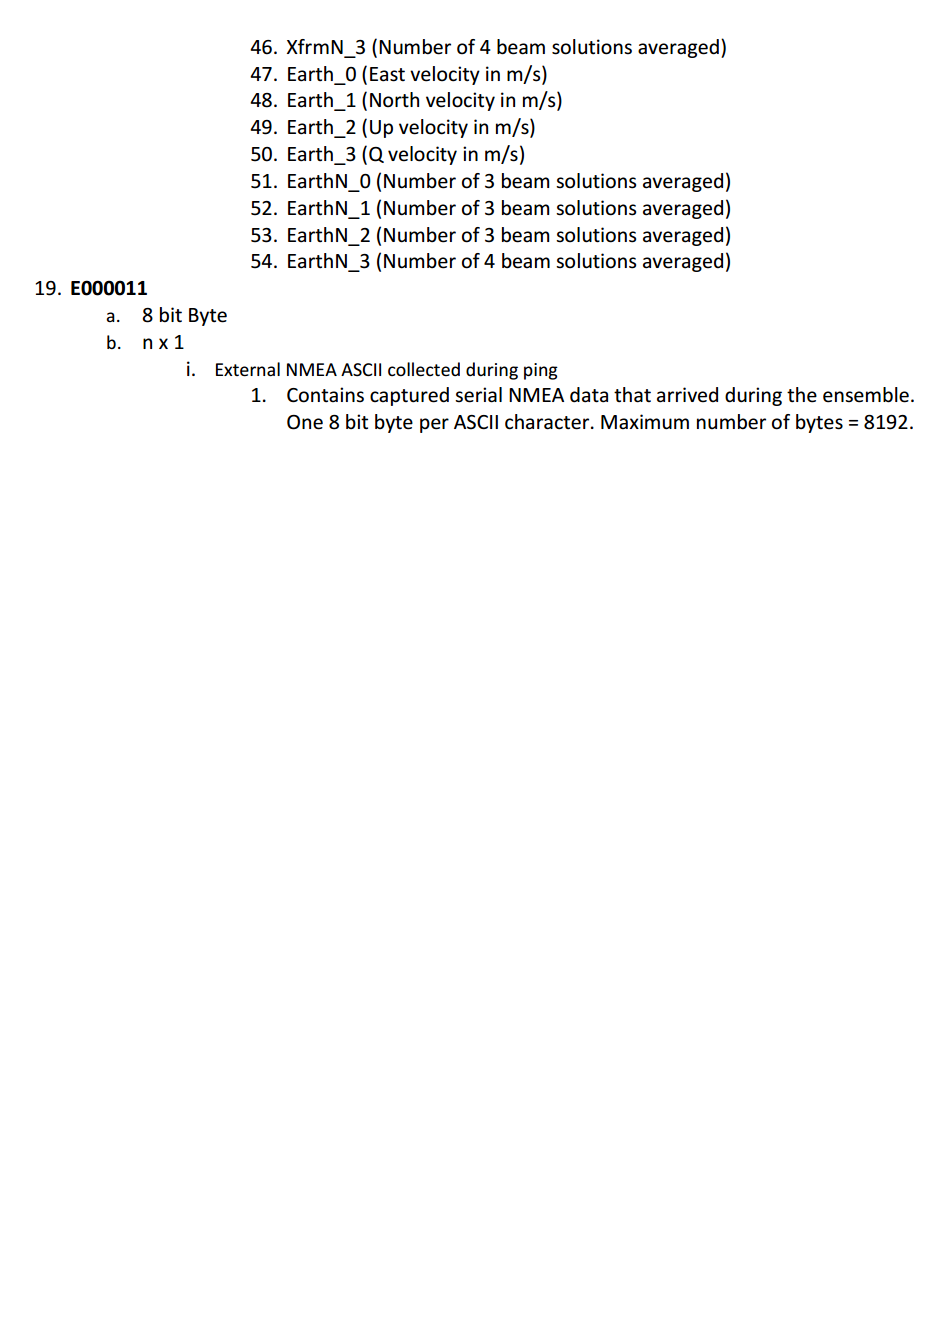
\includegraphics[width=1\textwidth]{ens6}
\end{figure}
\begin{figure}[ht]
\centering
      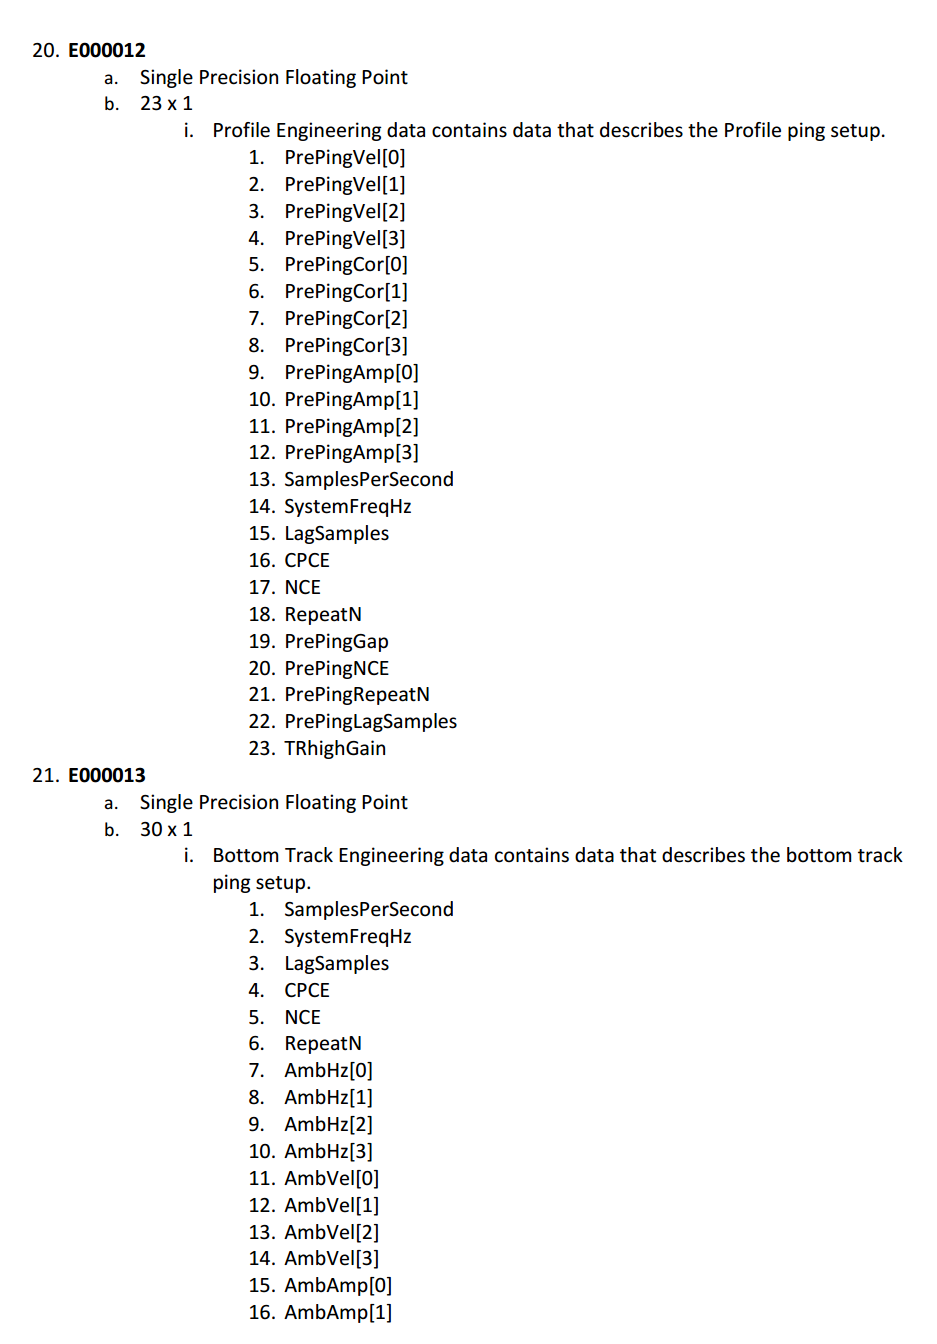
\includegraphics[width=1\textwidth]{ens7}
\end{figure}
\begin{figure}[ht]
\centering
      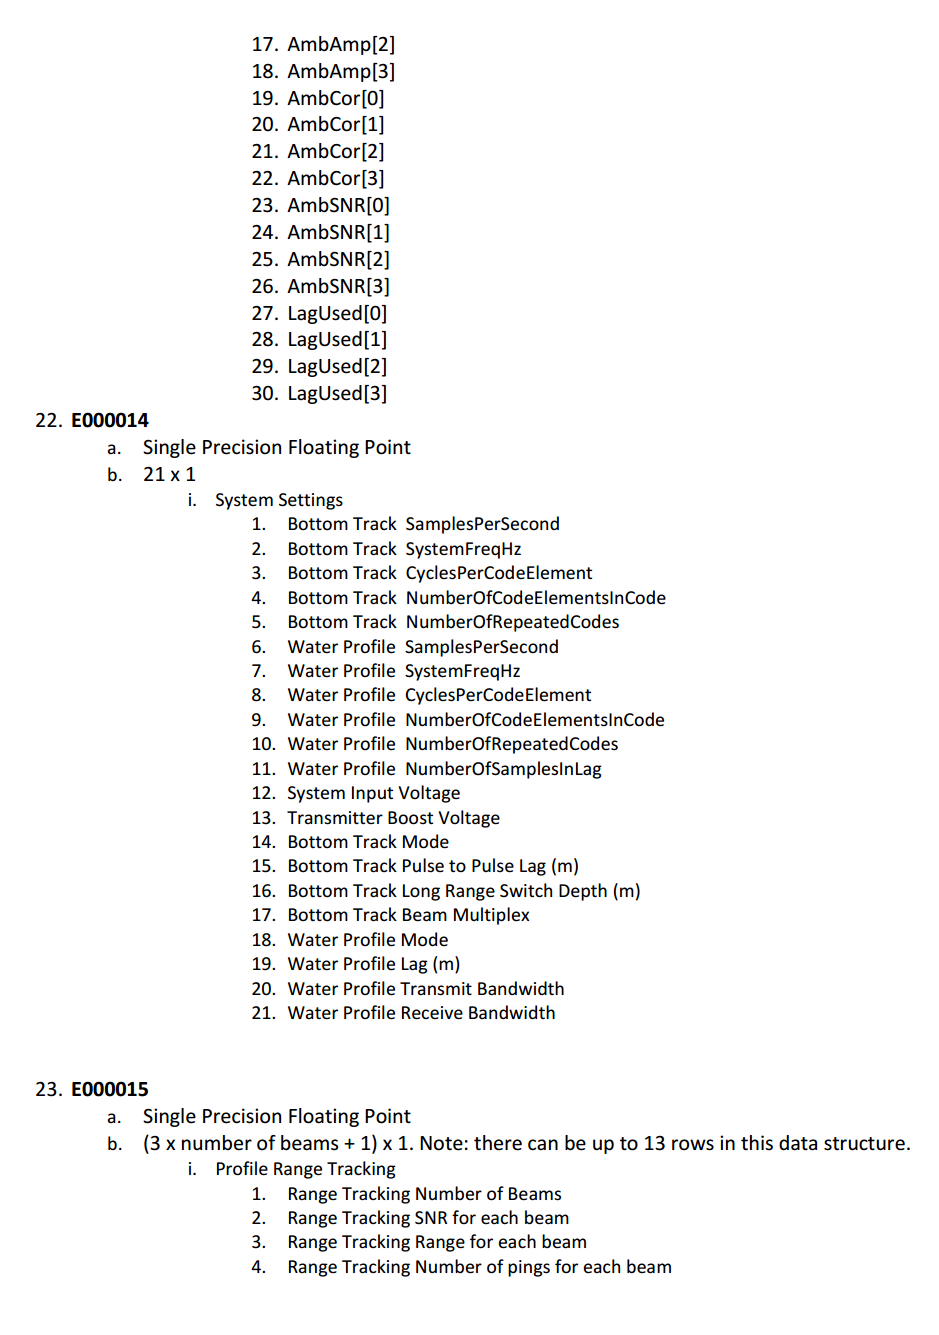
\includegraphics[width=1\textwidth]{ens8}
\end{figure}

\chapter{ADCP Burst Generator}
The source code used to generate ADCP bursts, and send them over a serial port.
\lstset{basicstyle=\tiny}
\begin{lstlisting}[language=C++]
/********************************************************
 * File:   createBurst.h
 * Author: Christian Ott
 * Created on April 15, 2016
 *
 * Copyright (c) 2016, General Acoustics e.K.
 * Redistribution and use in source and binary forms, with or without modification, are permitted!
 *
 * 2016-06-29 v1.00: First Release
 *
 * *****************************************************/

#ifndef ADCP_LOGGER_CREATEBURST_H
#define ADCP_LOGGER_CREATEBURST_H

#include <vector>
#include <chrono>
#include "../src/AdcpDataSet.h"
#include "../src/AdcpLogger.h"
#include "../src/MatlabUtils.h"

using ByteVec = std::vector<unsigned char >;
using TimeStamp = std::chrono::system_clock::time_point;
using Int32Vec = std::vector<int32_t>;
using Float32Vec = std::vector<boost::float32_t>;
using MessageVec = std::vector<BinaryMessage>;
struct ErrorConfig{
    int doubleheader;
    int doublestartseq;
    int startseqshort;
    int halfens;
    int missingbyte;
};

MessageVec createBurst(uint32_t stertEnsNr, TimeStamp ts, uint32_t numOfEns, ErrorConfig err );

ByteVec createSmallFrame(TimeStamp ts, uint32_t ensNr);
ByteVec createBigFrame(TimeStamp ts, uint32_t ensNr);

static Int32Vec generateRandomIntVec(size_t size);
static Float32Vec generateRandomFloatVec(size_t size);

#endif //ADCP_LOGGER_CREATEBURST_H

\end{lstlisting}
\pagebreak

\begin{lstlisting}[language=C++]
/********************************************************
 * File:   createBurst.cpp
 * Author: Christian Ott
 * Created on April 15, 2016
 *
 * Copyright (c) 2016, General Acoustics e.K.
 * Redistribution and use in source and binary forms, with or without modification, are permitted!
 *
 * 2016-06-29 v1.00: First Release
 *
 * *****************************************************/
#include <boost/thread.hpp>
#include "createBurst.h"
#include "../src/AdcpLogger.h"
#include "../external/SerialPort.h"
#include "../src/BinaryIO.h"
void runOutput(std::string com, uint32_t baud, MessageQueue &istream);
void runGenerator(MessageQueue &istream);
ByteVec createSmallFrame(TimeStamp ts, uint32_t ensNr);
ByteVec createBigFrame(TimeStamp ts, uint32_t ensNr);
MessageVec createBurst(uint32_t stertEnsNr, TimeStamp ts, uint32_t numOfEns, uint32_t delta, bool err );

int main(int argc, char* argv[]) {

    moodycamel::ConcurrentQueue<BinaryMessage, moodycamel::ConcurrentQueueDefaultTraits> MessageQueue(200);

    std::string com = argv[1];
    uint32_t baud =  std::stoi(argv[2]);

    boost::thread ensGenerator(runGenerator,std::ref(MessageQueue));
    boost::thread outputThread(runOutput, com, baud, std::ref(MessageQueue));

    ensGenerator.join();
    outputThread.join();
}
void runOutput(std::string com, uint32_t baud, MessageQueue &istream){
    SerialPort serial(com,baud);

    bool exitLoop = false;
    moodycamel::ConsumerToken ct(istream);
    while(!exitLoop){
        BinaryMessage msg;
        if(istream.try_dequeue(ct,msg)) {
            serial.write((const char *) &msg.getDataP()->data()[0], msg.getDataP()->size());
        }
    }
    serial.close();
}

void runGenerator(MessageQueue &istream){
    auto ts = TimeUtils::string_to_time_point("2016-06-15 02:02:00.00");
    auto ensnr = 20;
    while(1){

        auto burst = createBurst(ensnr,ts,2048,200,false);
        for(auto b : burst){
            istream.enqueue(b);
            boost::this_thread::sleep(boost::posix_time::milliseconds(2));
        }
        boost::this_thread::sleep(boost::posix_time::seconds(20));
        ts += std::chrono::minutes(10);
        ensnr +=2048;
    }
}
MessageVec createBurst(uint32_t stertEnsNr, TimeStamp ts, uint32_t numOfEns, uint32_t delta, bool err ){
    auto ensnr = stertEnsNr;
    auto tts = ts;
    std::random_device rd;     // only used once to initialise (seed) engine
    std::mt19937 rng(rd());    // random-number engine used (Mersenne-Twister in this case)
    std::uniform_int_distribution<int> uni(1,numOfEns); // guaranteed unbiased

    auto rand = uni(rng);
    MessageVec vec;

    while( numOfEns > 0){
        ByteVec frame;
        if((numOfEns % 2) == 0){
            frame = createSmallFrame(tts, ensnr);
        } else{
            frame = createBigFrame(tts, ensnr);
        }

        if (numOfEns == rand && err) {
            frame.insert(frame.begin(),frame.begin(),frame.begin()+32);
        }
        BinaryMessage m(tts,std::move(frame));
        vec.push_back(std::move(m));
        ensnr++;
        tts += std::chrono::milliseconds(delta);
        numOfEns--;
    }
    return std::move(vec);
}


ByteVec createSmallFrame(TimeStamp ts, uint32_t ensNr){
    AdcpEnsemble ensemble;
    ensemble.matrices.insert({"E000001", std::make_shared<E01>()});
    std::dynamic_pointer_cast<ExxFloat32>(ensemble.matrices["E000001"])->setVector(
            generateRandomFloatVec(30),
            30,
            1);


    ensemble.matrices.insert({"E000004", std::make_shared<E04>()});
    std::dynamic_pointer_cast<ExxFloat32>(ensemble.matrices["E000004"])->setVector(
            generateRandomFloatVec(30),
            30,
            1);

    ensemble.matrices.insert({"E000005", std::make_shared<E05>()});
    std::dynamic_pointer_cast<ExxFloat32>(ensemble.matrices["E000005"])->setVector(
            generateRandomFloatVec(30),
            30,
            1);

    ensemble.matrices.insert({"E000006", std::make_shared<E06>()});
    std::dynamic_pointer_cast<ExxInt32>(ensemble.matrices["E000006"])->setVector(
            generateRandomIntVec(30),
            30,
            1);

    auto e8vec = generateRandomIntVec(23);
    e8vec[0] = ensNr;
    e8vec[1] = 30;
    e8vec[2] = 1;
    auto ts_time = std::chrono::system_clock::to_time_t(ts);
    auto ts_sec = std::chrono::system_clock::from_time_t(ts_time);
    std::chrono::milliseconds ms = std::chrono::duration_cast<std::chrono::milliseconds>(ts - ts_sec);
    std::tm * ttm = localtime(&ts_time);

    e8vec[6] = ttm->tm_year+1900;
    e8vec[7] = ttm->tm_mon+1;
    e8vec[8] = ttm->tm_mday;

    e8vec[9] = ttm->tm_hour;
    e8vec[10] = ttm->tm_min;
    e8vec[11] = ttm->tm_sec;

    e8vec[12] = ms.count()/10;
    ensemble.matrices.insert({"E000008", std::make_shared<E08>()});
    std::dynamic_pointer_cast<ExxInt32>(ensemble.matrices["E000008"])->setVector(
            std::move(e8vec),
            23,
            1);

    ensemble.matrices.insert({"E000009", std::make_shared<E09>()});
    std::dynamic_pointer_cast<ExxFloat32>(ensemble.matrices["E000009"])->setVector(
            generateRandomFloatVec(13),
            13,
            1);

    ensemble.matrices.insert({"E000014", std::make_shared<E14>()});
    std::dynamic_pointer_cast<ExxFloat32>(ensemble.matrices["E000014"])->setVector(
            generateRandomFloatVec(23),
            23,
            1);

    ensemble.matrices.insert({"E000015", std::make_shared<E15>()});
    std::dynamic_pointer_cast<ExxFloat32>(ensemble.matrices["E000015"])->setVector(
            generateRandomFloatVec(4),
            4,
            1);

    AdcpConverter converter;
    auto frame = converter.ensembleToFrame(&ensemble);
    ByteVec res;
    frame.toByte(&res);
    return std::move(res);
}


ByteVec createBigFrame(TimeStamp ts, uint32_t ensNr){
    AdcpEnsemble ensemble;
    ensemble.matrices.insert({"E000001", std::make_shared<E01>()});
    std::dynamic_pointer_cast<ExxFloat32>(ensemble.matrices["E000001"])->setVector(
            generateRandomFloatVec(30*4),
            30,
            4);

    ensemble.matrices.insert({"E000002", std::make_shared<E02>()});
    std::dynamic_pointer_cast<ExxFloat32>(ensemble.matrices["E000002"])->setVector(
            generateRandomFloatVec(30*4),
            30,
            4);

    ensemble.matrices.insert({"E000003", std::make_shared<E03>()});
    std::dynamic_pointer_cast<ExxFloat32>(ensemble.matrices["E000003"])->setVector(
            generateRandomFloatVec(30*4),
            30,
            4);

    ensemble.matrices.insert({"E000004", std::make_shared<E04>()});
    std::dynamic_pointer_cast<ExxFloat32>(ensemble.matrices["E000004"])->setVector(
            generateRandomFloatVec(30*4),
            30,
            4);

    ensemble.matrices.insert({"E000005", std::make_shared<E05>()});
    std::dynamic_pointer_cast<ExxFloat32>(ensemble.matrices["E000005"])->setVector(
            generateRandomFloatVec(30*4),
            30,
            4);

    ensemble.matrices.insert({"E000006", std::make_shared<E06>()});
    std::dynamic_pointer_cast<ExxInt32>(ensemble.matrices["E000006"])->setVector(
            generateRandomIntVec(30*4),
            30,
            4);

    ensemble.matrices.insert({"E000007", std::make_shared<E07>()});
    std::dynamic_pointer_cast<ExxInt32>(ensemble.matrices["E000007"])->setVector(
            generateRandomIntVec(30*4),
            30,
            4);

    auto e8vec = generateRandomIntVec(23);
    e8vec[0] = ensNr;
    e8vec[1] = 30;
    e8vec[2] = 4;

    auto ts_time = std::chrono::system_clock::to_time_t(ts);
    auto ts_sec = std::chrono::system_clock::from_time_t(ts_time);
    std::chrono::milliseconds ms = std::chrono::duration_cast<std::chrono::milliseconds>(ts - ts_sec);
    std::tm * ttm = localtime(&ts_time);

    e8vec[6] = ttm->tm_year+1900;
    e8vec[7] = ttm->tm_mon+1;
    e8vec[8] = ttm->tm_mday;

    e8vec[9] = ttm->tm_hour;
    e8vec[10] = ttm->tm_min;
    e8vec[11] = ttm->tm_sec;

    e8vec[12] = ms.count()/10;
    ensemble.matrices.insert({"E000008", std::make_shared<E08>()});
    std::dynamic_pointer_cast<ExxInt32>(ensemble.matrices["E000008"])->setVector(
            std::move(e8vec),
            23,
            1);

    ensemble.matrices.insert({"E000009", std::make_shared<E09>()});
    std::dynamic_pointer_cast<ExxFloat32>(ensemble.matrices["E000009"])->setVector(
            generateRandomFloatVec(13),
            13,
            1);

    ensemble.matrices.insert({"E000014", std::make_shared<E14>()});
    std::dynamic_pointer_cast<ExxFloat32>(ensemble.matrices["E000014"])->setVector(
            generateRandomFloatVec(21),
            21,
            1);
    ensemble.matrices.insert({"E000015", std::make_shared<E15>()});
    std::dynamic_pointer_cast<ExxFloat32>(ensemble.matrices["E000015"])->setVector(
            generateRandomFloatVec(13),
            13,
            1);
    AdcpConverter converter;
    auto frame = converter.ensembleToFrame(&ensemble);
    ByteVec res;
    frame.toByte(&res);
    return std::move(res);
}
static Int32Vec generateRandomIntVec(size_t size){
    using value_type = int32_t ;
    // We use static in order to instantiate the random engine
    // and the distribution once only.
    // It may provoke some thread-safety issues.
    static std::uniform_int_distribution<value_type> distribution(
            0,
            10);
    static std::default_random_engine generator;

    std::vector<value_type> data(size);
    std::generate(data.begin(), data.end(), []() { return distribution(generator); });
    return data;
}


static Float32Vec generateRandomFloatVec(size_t size){
    using value_type = boost::float32_t ;
    // We use static in order to instantiate the random engine
    // and the distribution once only.
    // It may provoke some thread-safety issues.
    boost::float32_t min = -1.999f;
    boost::float32_t max = 1.999f;

    static std::uniform_real_distribution<value_type> distribution(
            min,
            max);
    static std::default_random_engine generator;

    std::vector<value_type> data(size);
    std::generate(data.begin(), data.end(), []() { return distribution(generator); });
    return data;
}
\end{lstlisting}
\chapter{Contents of the CD}
\begin{itemize}
\item\textbf{01\_source\_code} - Contains the final source code, as well as a small README in markdown and PDF.
\item\textbf{02\_tex\_report} - Contains the source code of the report, including the images and the final printed PDF.
\item\textbf{03\_presentation} - Contains the pptx from the final presentation.
\item \textbf{04\_other} - Contains various documents and files used for this project.
	\begin{itemize}
		\item \textbf{cd\_label} - The digital DC label used to print the CD's
		\item \textbf{documentation} - The documentation files used for the implementation	
		\item \textbf{measurements} - Measurement results with the according bat scripts
		\item \textbf{raw\_adcp\_data} - A few ADCP files, in case the software needs to be tested.
	\end{itemize}
\end{itemize}
